% !TEX encoding = UTF-8 Unicode
\documentclass[10pt,a4paper]{article}
\usepackage[T2A]{fontenc}
\usepackage[utf8]{inputenc}
\usepackage[intlimits]{amsmath}
\usepackage{amssymb}
\usepackage[russian,english]{babel}
\usepackage{framed}
\usepackage{graphicx}
\usepackage[usenames]{color}
\usepackage{colortbl}
\usepackage[dvipsnames]{xcolor}

\usepackage[left=2cm,right=2cm,top=2cm,bottom=2cm]{geometry}

\let\P\relax
\DeclareMathOperator{\P}{\mathbb{P}}
\DeclareMathOperator{\E}{\mathbb{E}}
\DeclareMathOperator{\Var}{\mathbb{V}\mathrm{ar}}
\DeclareMathOperator{\Cov}{\mathbb{C}\mathrm{ov}}


\begin{document}
\centering 
\pagecolor{Tan}
\begin{figure}[h]
\centering

\includegraphics[width=14cm]{all.jpg}
\end{figure}
\large{\textcolor{red}{Маленький} \textcolor{blue}{зоопарк} \textcolor{green}{дифференциальных} \textcolor{cyan}{уравнений}.} \\
\newpage
\pagecolor{cyan}
\begin{figure}[h]
\centering
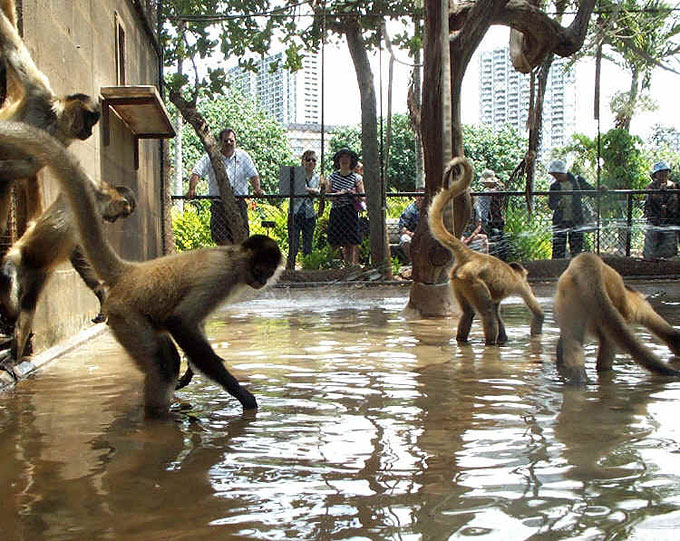
\includegraphics[width=12cm]{monkey.png}
\end{figure}
\par \textbf{Зверь 1.} Уравнения с разделяющимися уравнений.
\par Внешний вид: $f(x) \, dx = g(y) \, dy$.
\par Как решать: проинтегрировать правую и левую части.
\par \textbf{Пример:} $y' - 5y = 0$
\begin{eqnarray*}
y' - 5y = 0 \Rightarrow \frac{dy}{dx} = 5y \Rightarrow \frac{1}{y}dy = 5 dx  \text{ или } y = 0
\end{eqnarray*}
\begin{eqnarray*}
\int \frac{1}{y} \, dy = \int 5 \, dx \text{ или } y =0 \Rightarrow \log|y| = 5x + c, c \in \mathbb{R} \text{ или } y = 0
\end{eqnarray*}
\par \textbf{Ответ:} $y(x) = c \cdot e^{5x}, c \in \mathbb{R}$ \\
\newpage
\pagecolor{Apricot}
\begin{figure}[h]
\centering
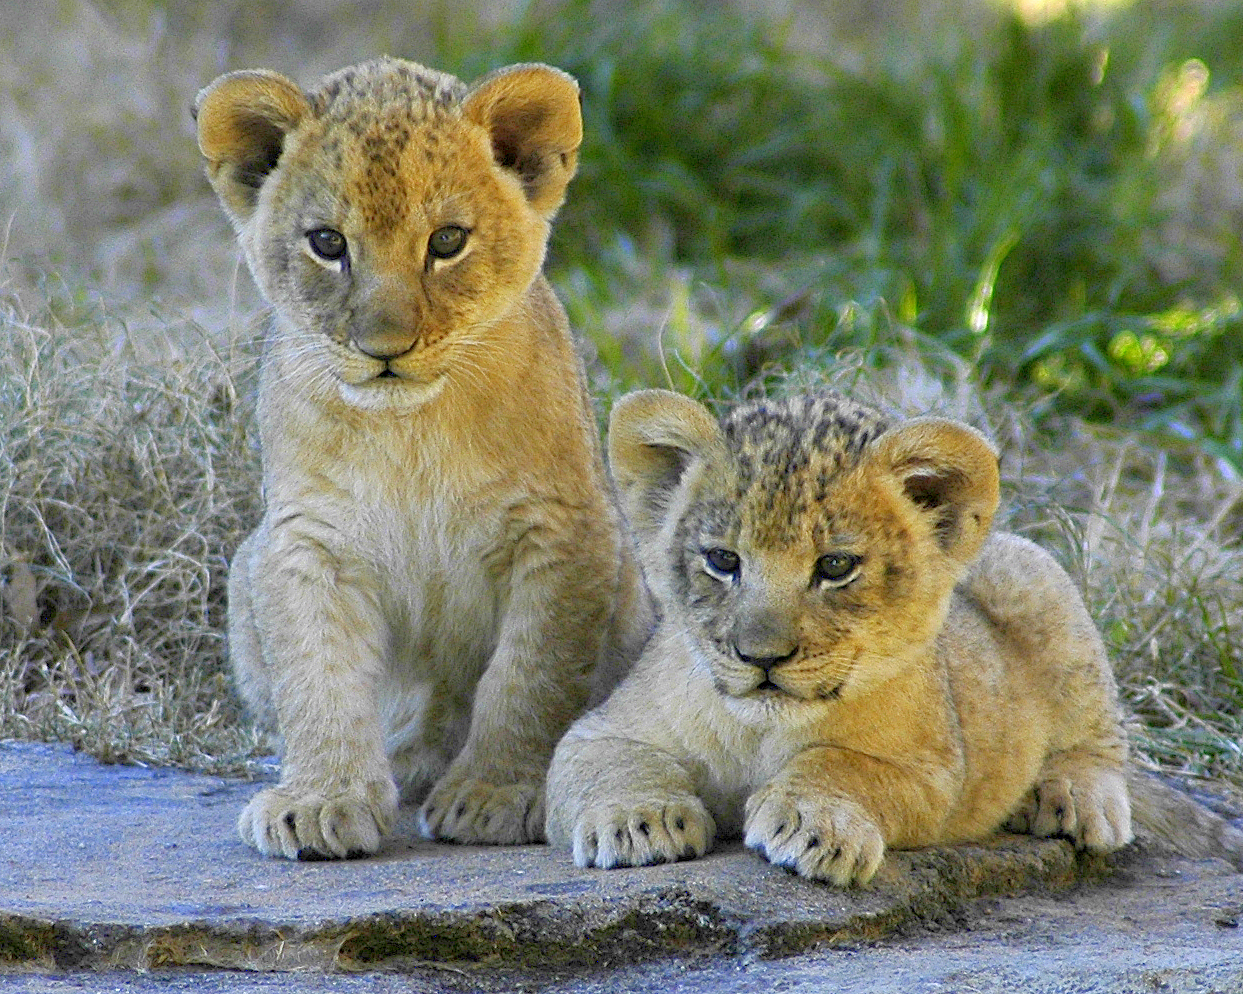
\includegraphics[width=12cm]{2cases.jpg}
\end{figure}
\par \textbf{Зверь 2.} Линейное уравнение первой степени с ненулевой правой частью.
\par Внешний вид: $y' + f(x) y = g(x)$.
\par Как решать: 
\par \textbf{Способ 1.} Educated guesswork. 
\par Шаг 1.
\par Заменить в исходном уравнении правую часть на ноль.
\par Решить однородное уравнение $y' + f(x) y = 0$. Здесь разделяются переменные.
\par Получается ответ в духе $y_{hom}(x) = c \cdot \dots$
\par Шаг 2.
\par По виду правой части угадать решение, $y_{pi}(x).$
\par Если в правой части содержится $\sin (x)$, значит в решении есть $a \cdot \cos(x) + b \cdot \sin(x)$.
\par Нюанс:
\par Если угадываемый вид содержится в $y_{hom}(x)$, то догадку следует домножить на $x$.
\par Записываем ответ в виде $y(x) = y_{hom}(x) + y_{pi}(x)$
\par \textbf{Пример 1:} $y' - 5y = 10$
\par Шаг 1.
\par Решаем $y' - 5y = 0$. Уже делали, $y_{hom}(x) = ce^{5x}$.
\par Шаг 2.
\par $RHS = 10.$ Кто еще не в курсе, RHS - это <<Right Hand Side>>.
\par $10$ - это константа, поэтому будем искать частное решение $y_{pi}$ в виде $y = a$. 
\par Тогда $y' = 0$. Подставим предположенные $y$ и $y'$ в уравнение.
\par Получаем $0 - 5a  = 10$, значит $a = -2.$ 
\par \textbf{Ответ:} $y(x) = c \cdot e^{5x} - 2, c \in \mathbb{R}$
\par \textbf{Пример 2:} $y' - 5y = 6e^{5x}$
\par Шаг 1.
\par Решаем $y' - 5y = 0$. Уже делали, $y_{hom}(x) = ce^{5x}$.
\par Шаг 2.
\par $RHS = 6e^{5x}.$ 
\par Будем искать частное решение $y_{pi}$ в виде $y = a \cdot e^{5x}$. 
\par Ого! Такое уже входит в $y_{hom}(x)$. Поэтому домножаем догадку на $x$.
\par Значит $y = a \cdot x \cdot e^{5x}$, тогда $y' = a \cdot e^{5x} + 5ax \cdot e^{5x}$
\par Подставим предположенные $y$ и $y'$ в уравнение.
\par Получаем $a \cdot e^{5x} + 5ax \cdot e^{5x} - 5a \cdot x \cdot e^{5x}  = 6e^{5x}$, после упрощения: $a \cdot e^{5x} = 6e^{5x}$, значит $a = 6.$ 
\par \textbf{Ответ:} $y(x) = c \cdot e^{5x} + 6x e^{5x}, c \in \mathbb{R}$
\par \textbf{Способ 2.} Variation of constant.
\par Метод вариации постоянной, что-то в духе <<изменение неизменного>> 
\par Шаг 1.
\par Заменить в исходном уравнении правую часть на ноль.
\par Решить однородное уравнение $y' + f(x) y = 0$. Здесь разделяются переменные.
\par Получается ответ в духе $y_{hom}(x) = c \cdot \dots$
\par Шаг 2.
\par Сделать вид, что $c$ - не просто константа, а функция $c(x)$.
\par Подставить полученное решение в исходное уравнение и найти эту $c(x)$.
\par \textbf{Пример:} $y' - 5y = 6e^{5x}$
\par Шаг 1.
\par Решаем $y' - 5y = 0$. Уже делали, $y_{hom}(x) = ce^{5x}$.
\par Шаг 2.
\par Ищем решение в виде $y(x) = c(x) e^{5x}$
\par Тогда $y'(x) = 5c(x) e^{5x} + c'(x)e^{5x}$
\par Подставляем $y(x)$ и $y'(x)$ в исходное уравнение:
\begin{eqnarray*}
5x(x) e^{5x} + c'(x) e^{5x} - 5c(x)e^{5x} = 6e^{5x} \Rightarrow c'(x) = 6 \text{ или } c(x) = 6x + c
\end{eqnarray*}
\par \textbf{Ответ:} $y(x) = (6x + c) \cdot e^{5x}, c \in \mathbb{R}$ \\
\newpage{}
\pagecolor{magenta}
\begin{figure}[h]
\centering
\includegraphics[width=11cm]{hippo.jpg}
\end{figure}
\par \textbf{Зверь 3.} В полных дифференциалах.
\par Внешний вид: $A(x, y) \, dx + B(x,y) \, dy = 0, \frac{\partial{A}}{\partial{y}} = \frac{\partial{B}}{\partial{x}}$.
\par Как решать:<<Four step procedure>>
\begin{enumerate}
\item Сначала убедитесь, что это оно. Проверьте, что $\frac{\partial{A}}{\partial{y}} = \frac{\partial{B}}{\partial{x}}$
\item Представьте решение в виде $F(x,y) = \int A(x,y) \, dx + c(y)$
\item Возьмите $\frac{\partial{F(x,y)}}{\partial{y}}$ и приравняйте к $B(x,y)$.
\item Из полученного уравнения найдите $c(y)$.
\end{enumerate}
\par Не забудьте записать ответ $F(x,y) = 0$
\par \textbf{Пример:} $(2x - y) \, dx + (2y - x) \, dy = 0$
\begin{enumerate}
\item Проверяем $\frac{\partial{(2x-y)}}{\partial{y}} = \frac{\partial{(2y-x)}}{\partial{x}}$. OK!
\item $F(x,y) = \int 2x - y \, dx + c(y) = x^2 - xy + c(y)$
\item $\frac{\partial{(x^2 - xy + c(y))}}{\partial{y}} = 2y - x$
\par Получили уравнение: $ -x + c'(y) = 2y - x$
\item Решаем $c'(y) = 2y, c(y) = y^2 + c$
\end{enumerate}
\par \textbf{Ответ:} $x^2 - xy + y^2 + c = 0, c \in \mathbb{R}$ \\
\par \textbf{Зверь 3, неодомашненный, дикий}.
\par Внешний вид: $A(x, y) \, dx + B(x,y) \, dy = 0$, без всяких условий на $A(x,y)$ и $B(x,y)$!
\par Теорема об одомашнивании. Всегда найдется функция $r(x,y)$, такая, что после домножения на нее будет выполнятся условие $\frac{\partial{A}}{\partial{y}} = \frac{\partial{B}}{\partial{x}}$.
\par На практике найти этот integrating factor сложно, поэтому теорема имеет небольшой практический смысл. \\
\par \textbf{Небольшое предложение:} все-таки дикого зверя можно одомашнить, если
он не агрессивен, - можно найти интегрирующий множитель, проверив,
является ли разность производных функций-коэффициентов при dx и dy,
делённая на одну из этих функций в зависимости от порядка вычитания,
функцией лишь от одной переменной. Если да, то зверь не опасен.
\newpage
\pagecolor{JungleGreen}
\begin{figure}[h]
\centering
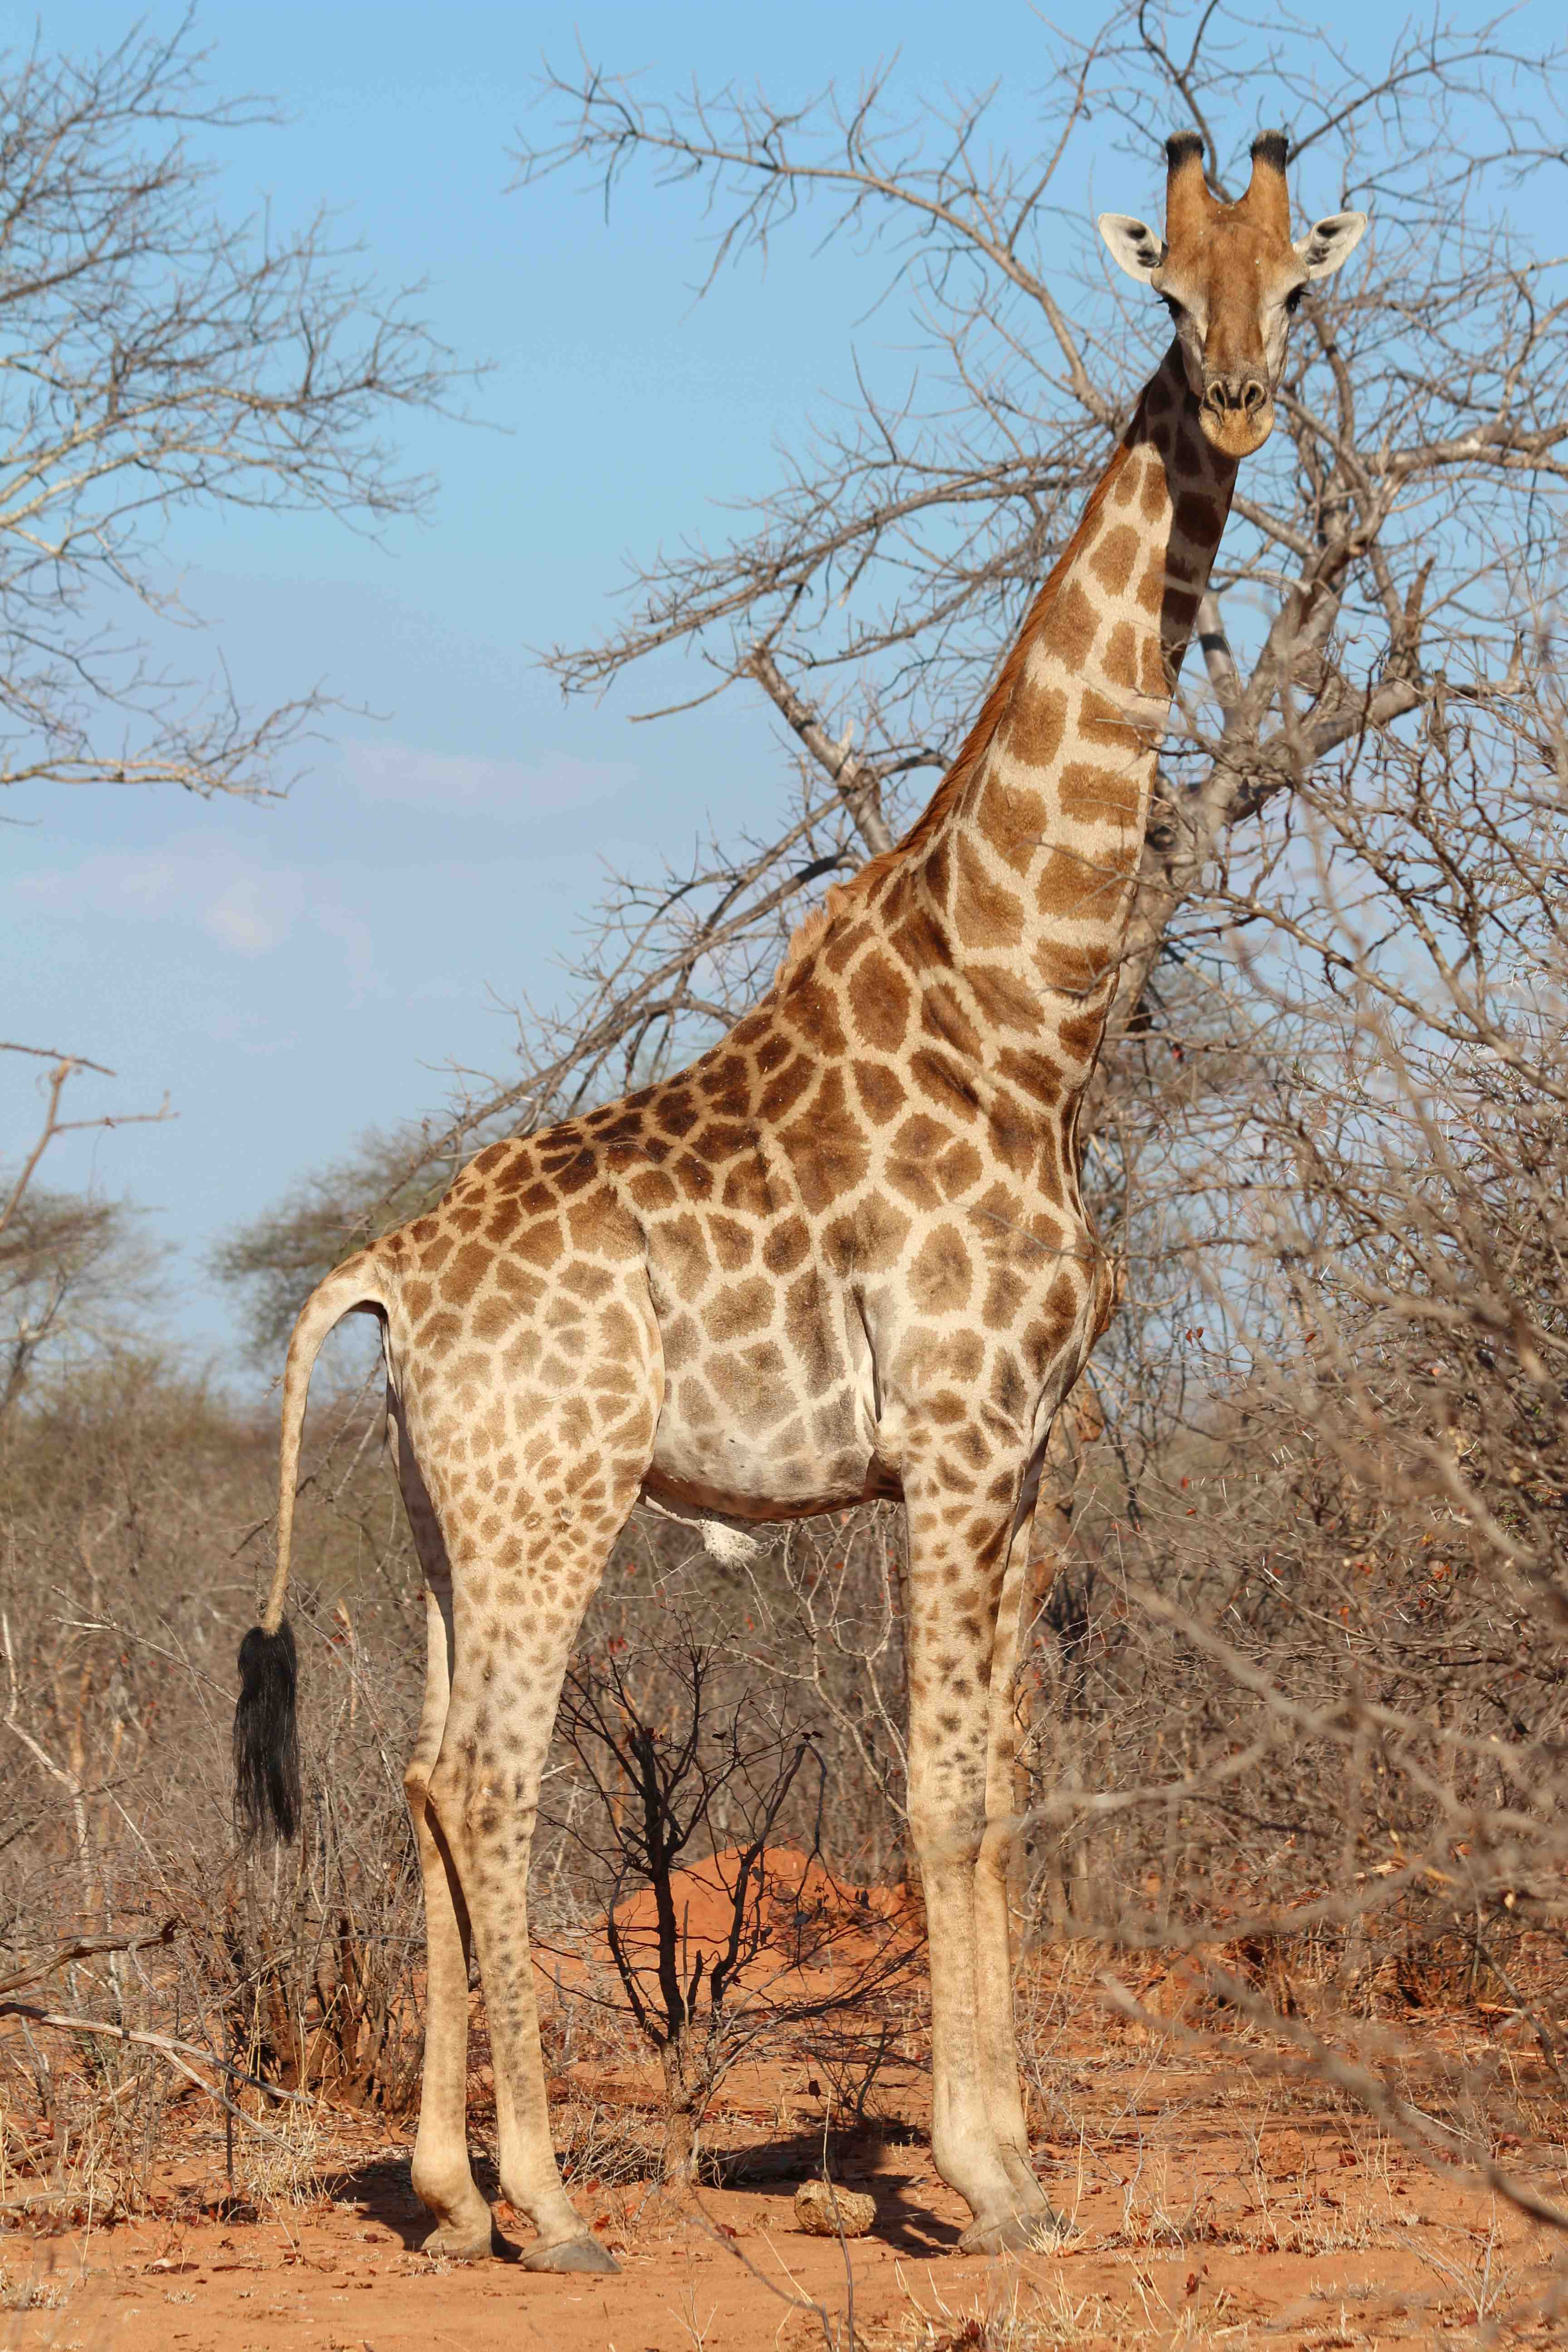
\includegraphics[width = 11cm]{giraffe.jpg}
\end{figure}
\par \textbf{Зверь 4.} Однородное по x и y.
\par Внешний вид: $A(x, y) \, dx + B(x,y) \, dy = 0$,  где $A(x,y)$ и $B(x,y)$ - однородные функции одной степени.
\par Как решать? Часто помогает замена $y(x) = x \cdot r(x)$.
\par При этому $dy$ заменяется на $xdr + rdx$. А, кстати, почему?
\par \textbf{Пример:} $x \, dy + (y+x) \, dx = 0$
\par Перед $dy$ и $dx$ стоят однородные функции первой степени.
\par Делаем замену: $y(x) = xr(x), dy = xdr + rdx $
\begin{eqnarray*}
x(xdr + rdx) + (xr + x) dx = 0 \Rightarrow xdr + (2r+1)dx = 0 
\end{eqnarray*}
\par Тут разделяются переменные.
\begin{eqnarray*}
\frac{1}{2r + 1} dr = -\frac{1}{x} dx \Rightarrow \frac{1}{2}\log|2r + 1| = -\log|x| + c
\end{eqnarray*}
\par Возвращаемся к $y$:
\par \textbf{Ответ:} $\log|2\frac yx + 1| = -2\log|x| + c, c \in \mathbb{R}$ \\
\newpage
\pagecolor{Salmon}
\begin{figure}[h]
\centering
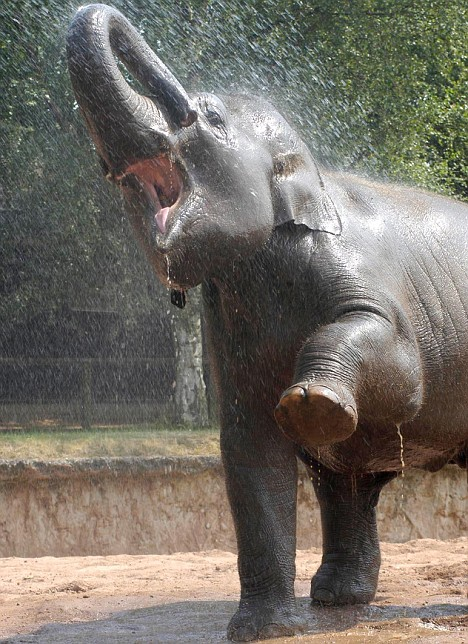
\includegraphics[width = 11cm]{eleph.jpg}
\end{figure}
\par \textbf{Зверь 5.} Уравнение Бернулли.
\par Внешний вид: $y' + f(x) y = g(x) y^n$,  
\par Как решать? Поделить уравнение на $y^n$ и сделать замену $r(x) = \frac1 {y(x)^{n-1}}$. 
\par При этом, конечно, $r' = - \frac{(n-1)y'}{y^n}$.
\par Получается линейное уравнение.
\par \textbf{Пример:} $y' - 5y = y^6$
\begin{eqnarray*}
\frac{y'}{y^6} - 5 \frac{1}{y^5} = 1 \text{ или } y = 0
\end{eqnarray*}
\begin{eqnarray*}
\frac{-5y'}{y^6} + 25 \frac{1}{y^5} = -5 \text{ или } y = 0
\end{eqnarray*}
\par Делаем замену $r(x) = \frac1 {y^5}$, при этом $r'(x) = \frac{-5y'}{y^6}$.
\par Получаем зверя под номером 2 --- $r' + 25r = -5$
\par Решаем: $r(x) = ce^{-25x} - \frac 1 5, c \in \mathbb{R}$.
\par Возвращаемся к $y$:
\par \textbf{Ответ:} $\frac 1 {y^5} = -ce^{-25x} - \frac 1 5, c \in \mathbb{R} \text{ или } y = 0$ \\
\newpage
\pagecolor{LimeGreen}
\begin{figure}[h]
\centering
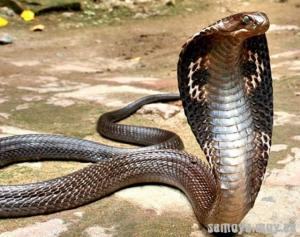
\includegraphics[width = 8cm]{snake.jpg}
\end{figure}
\par \textbf{Зверь 6.} Линейное уравнение произвольной степени с постоянными коэффициентами.
\par Внешний вид: $y^{(n)} + a_{n-1}y^{(n-1)} + \dots + a_1y' + a_0y = g(x)$
\par Как решать?
\par Шаг 1. Заменить в исходном уравнении правую часть на ноль.
\par Составить характеристическое уравнение:
\par $n$-ную производную $y$ заменить на $\lambda^n$
\par Найти корни: $\lambda_1, \dots, \lambda_n$
\par Записать решение однородного уравнения: $y_{hom}(x) = c_1e^{\lambda_1x} + \dots + c_ne^{\lambda_nx}$
\par Шаг 2. По виду правой части угадать решение, $y_{pi}(x).$
\par Записать ответ $y(x) = y_{hom}(x) + y_{pi}(x)$
\par \textbf{Пример:} $y'' - y' - 6y = 5e^{3x}$
\par Шаг 1.
\par Решаем $y'' - y' - 6y = 0$.
\par Составляем характеристическое уравнение: $\lambda^2 - \lambda - 6 = 0$
\par Находим корки: $\lambda_{1,2} = 3, -2$.
\par Значит $y_{hom}(x) = c_1e^{3x} + c_2e^{-2x}, c_{1,2} \in \mathbb{R}$
\par Шаг 2.
\par $RHS = 6e^{5x}.$ 
\par Будем искать частное решение $y_{pi}$ в виде $y = a \cdot e^{3x}$. 
\par Ого! Такое уже входит в $y_{hom}(x)$, домножаем догадку на $x$.
\par Стало быть ищем решение $y_{pi}(x) = axe^{3x}$
\par Значит $y' = a \cdot e^{3x} + 3axe^{3x}$ и $y'' = 3ae^{3x} + (3ae^{3x}+ 9axe^{3x}) = 6ae^{3x} + 9axe^{3x}$.
\par Подставим предположенные $y, y'$ и $y''$ в уравнение.
\par Получаем $6ae^{3x} + 9axe^{3x} - (a \cdot e^{3x} + 3axe^{3x}) - 6axe^{3x}  = 5e^{3x}$, после упрощения: $5a \cdot e^{3x} = 5e^{3x}$.
\par Значит $a = 1.$ 
\par \textbf{Ответ:} $y(x) = c_1e^{3x} + c_2e^{-2x} + xe^{3x}, c_{1, 2, 3} \in \mathbb{R}$ \\
\par Нюансы: 
\par \textbf{Комплексные корни.} Комплексные корни ходят парами: $\lambda_1 = a+ bi, \lambda_2 = a - bi$.
\par Им соответствует решение $(d_1 + d_2i)e^{\lambda_1 x} + (d_1 - d_2i)e^{\lambda_2 x}$.
\par Это же решение можно записать без мнимого $i$, зато с тригонометрией: $e^{ax}(c_1\cos(bx) + c_2\sin(bx))$
\par \textbf{Кратные корни.}
\par Если корень $\lambda$ встречается несколько раз, то:
\par Первому $\lambda_1 = \lambda$ соответсвует решение $e^{\lambda x}$
\par Второму $\lambda_2 = \lambda$ соответсвует решение $xe^{\lambda x}$
\par Третьему $\lambda_3 = \lambda$ соответсвует решение $x^2e^{\lambda x}$
\par И т.д.

\newpage
\pagecolor{YellowOrange}
\begin{figure}[h]
\centering
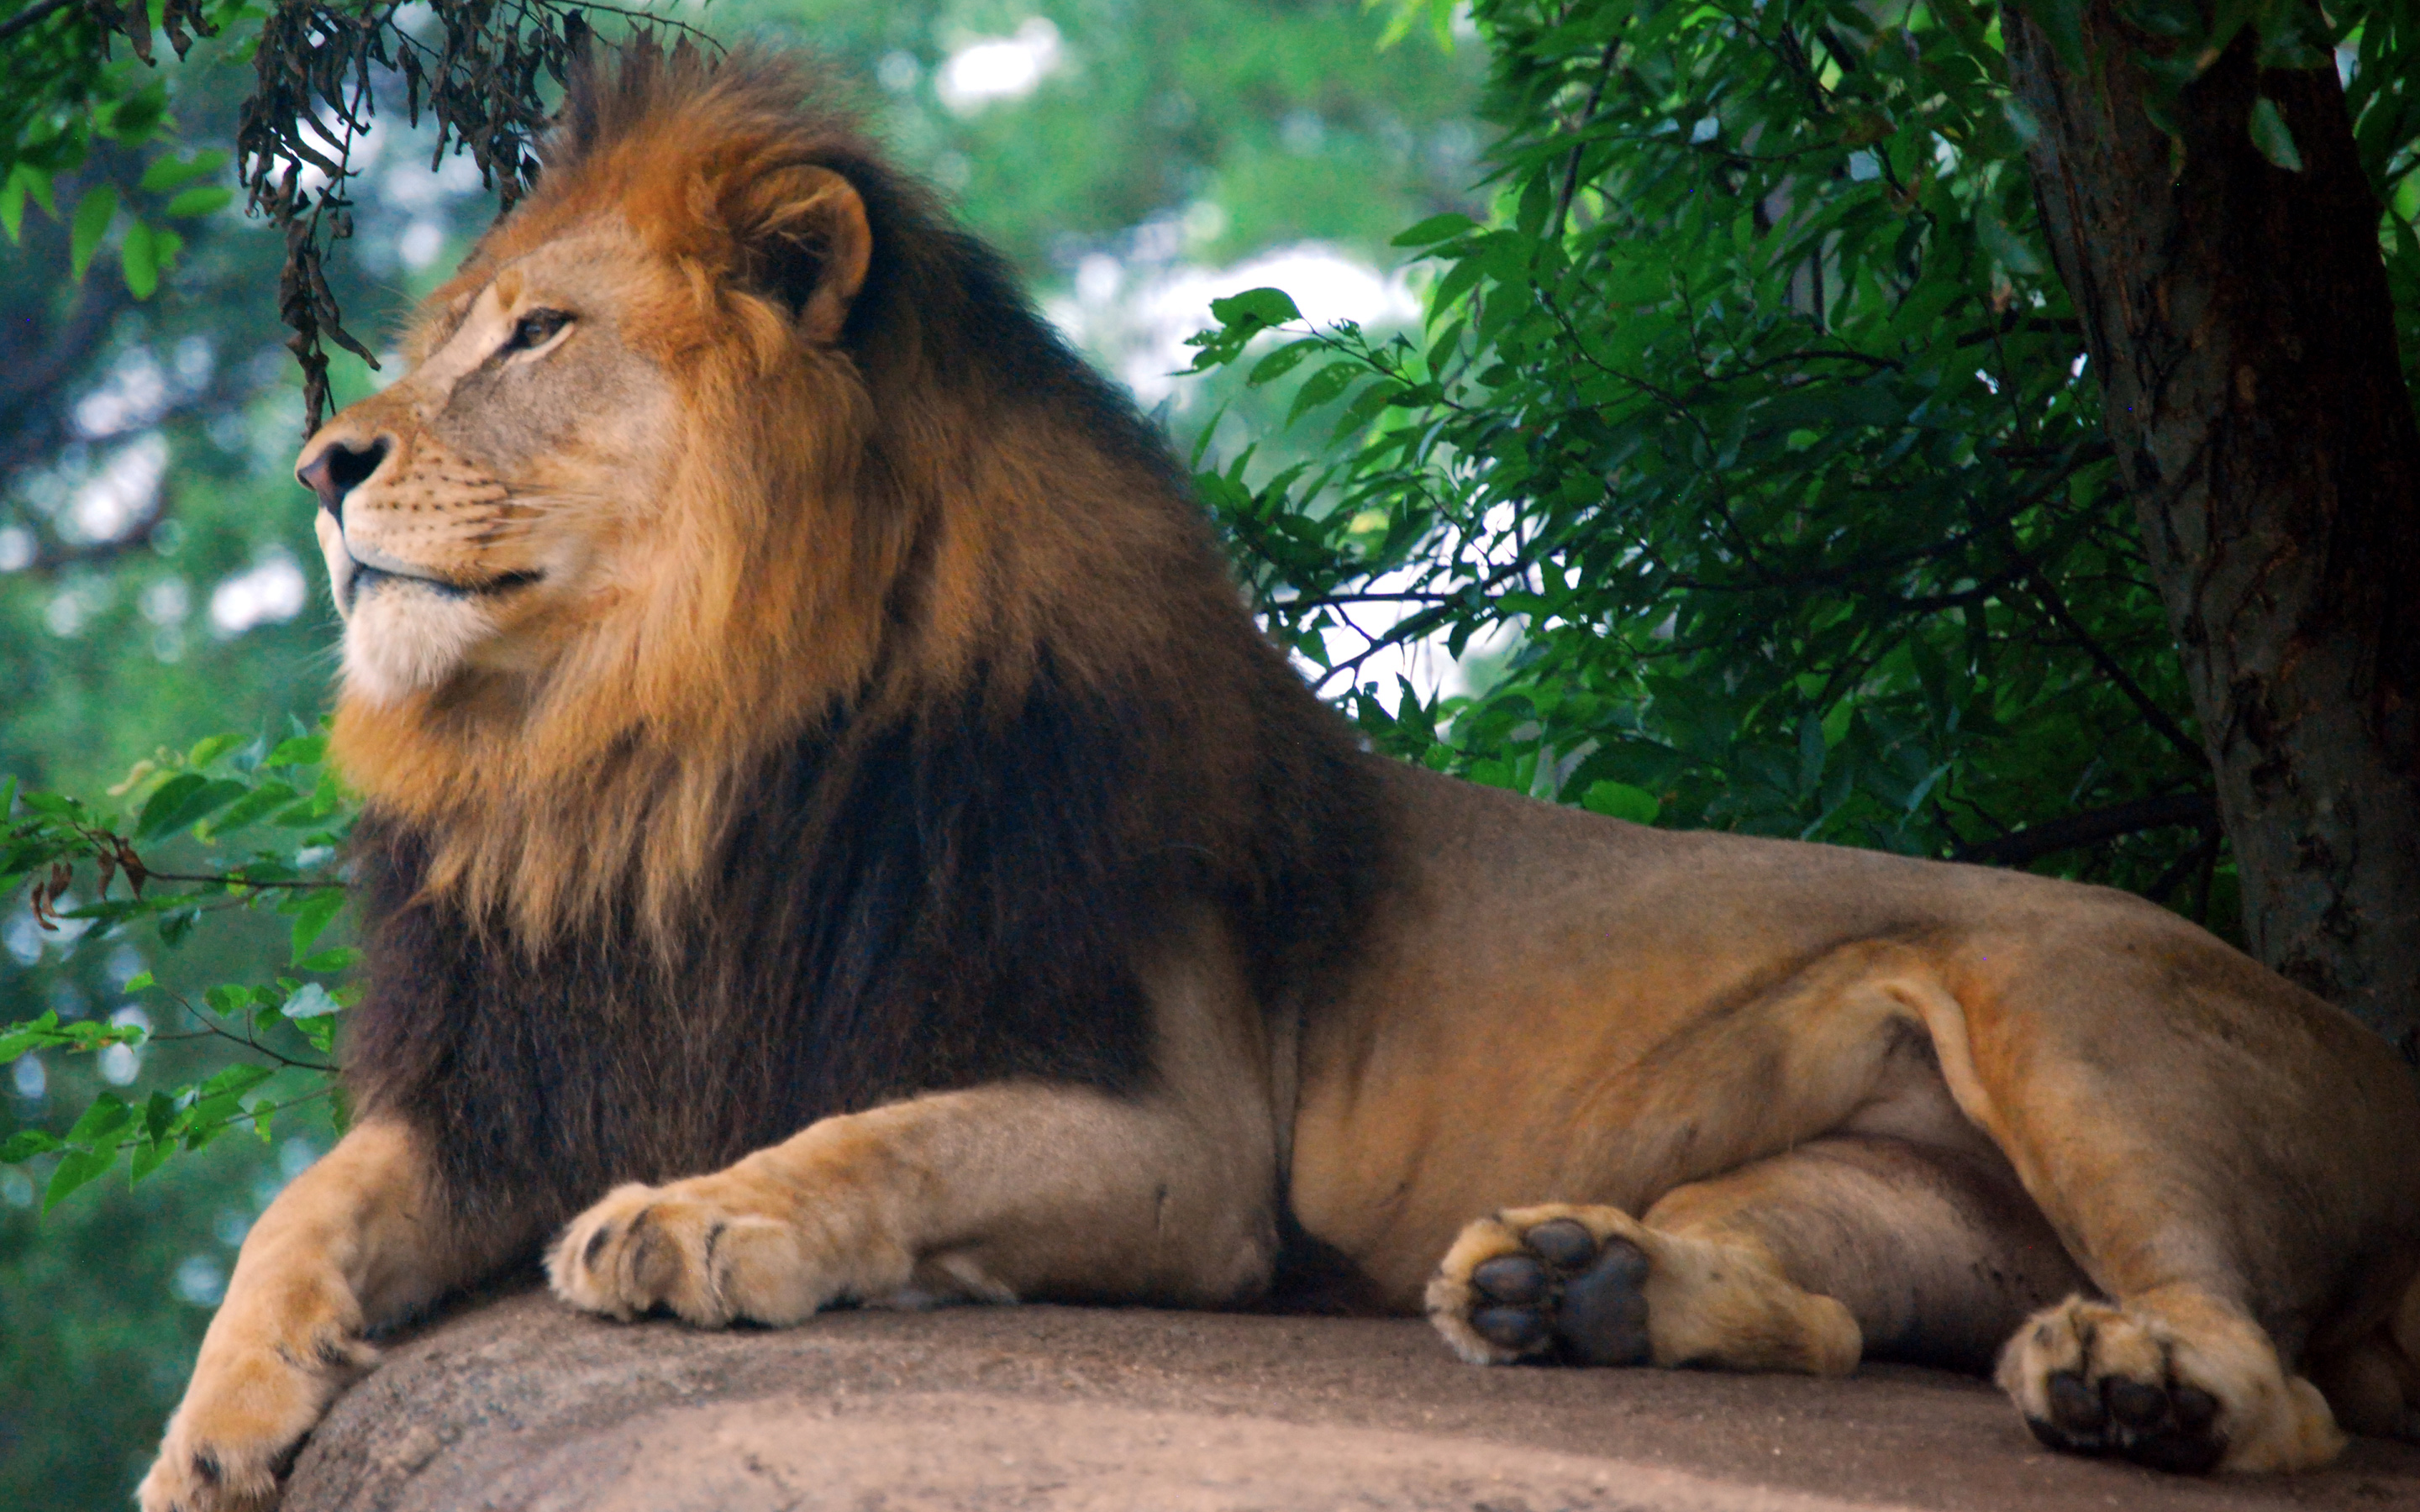
\includegraphics[width = 12cm]{king.jpg}
\end{figure}
\par Disclaimer:
\par Этот текст не претендует ни на полноту, ни на строгость, ни на безошибочность! 
\par Если есть вопросы, пожелания, комментарии, сообщения об ошибках, благодарности, то пишите на roah@yandex.ru. 
\par Борис Демешев \\

Благодарим Вас за посещение нашего зоопарка.
\end{document}
